\section{Database}
Til implementering af databasen samt kommunikation med denne benyttes programmet XAMPP. Programmet opretter en lokal apache webserver samt database på en given computer, der fungerer som et Localhost miljø. Den lokale webserver simulerer en ekstern webserver, hvilket giver et passende miljø til at teste og udvikle prototypen. Dertil anses dette ikke som værende fjernt fra et virkelighedsnært scenarie, hvor systemet benyttes med ekstern server og database.
Ved direkte håndtering af databasen benyttes phpMyAdmin, der er et online databaseadministrationssystem, som understøtter Structured Query Language (SQL) \cite{silbershatz2011}. 
Databasen er implementeret under navnet \textit{db\_KOL}, hvori tabeller oprettes på baggrund af design jf. \autoref{sec:ER} i relation til attributter og datatyper.

\subsection{Kommunikation med databasen}
*********** DB controller = PHP script!***********
Kommunikation mellem Android Studio og databasen kan ikke forekomme direkte, hvorfor php: Hypertext preprocessor scripts benyttes. Php er et Server-Side Scripting Language, hvilket køres på serveren og muliggør, at systemet kan tilgå databasen \cite{silbershatz2011}. 
Der er oprettet et php-script, \textit{config.php}, der indeholder informationerne host, bruger, adgangskode samt navn på den oprettede database. Dette script inkluderes i et seperat script, \textit{DB\_connect.php}, til at etablere forbindelsen til databasen. Der er opstillet forskellige php-scripts, som javakoden refererer til via URL links. Af disse links fremgår ip-adressen for serveren samt filplaceringen af det givne script. 

De forskellige scripts får information fra app'en for således at kunne udføre SQL-kommandoer. Informationen sendes fra app'en som en JavaScript Object Notation (JSON) repræsentation. JSON benyttes ved dataoverførsel, det er hertil muligt at pakke data som et objekt eller array.\cite{silbershatz2011} Php-scripts brugt i dette projekt er sat op til at tjekke, hvorvidt der bliver sendt en værdi i det respektive navn. Er værdierne sat og ikke NULL, ligges værdierne i en ny variabel. Et eksempel af dette ses af \autoref{fig:phplogind}, hvor et udklip af php-scriptet for log ind er visualiseret. 

\begin{figure} [H]
\centering
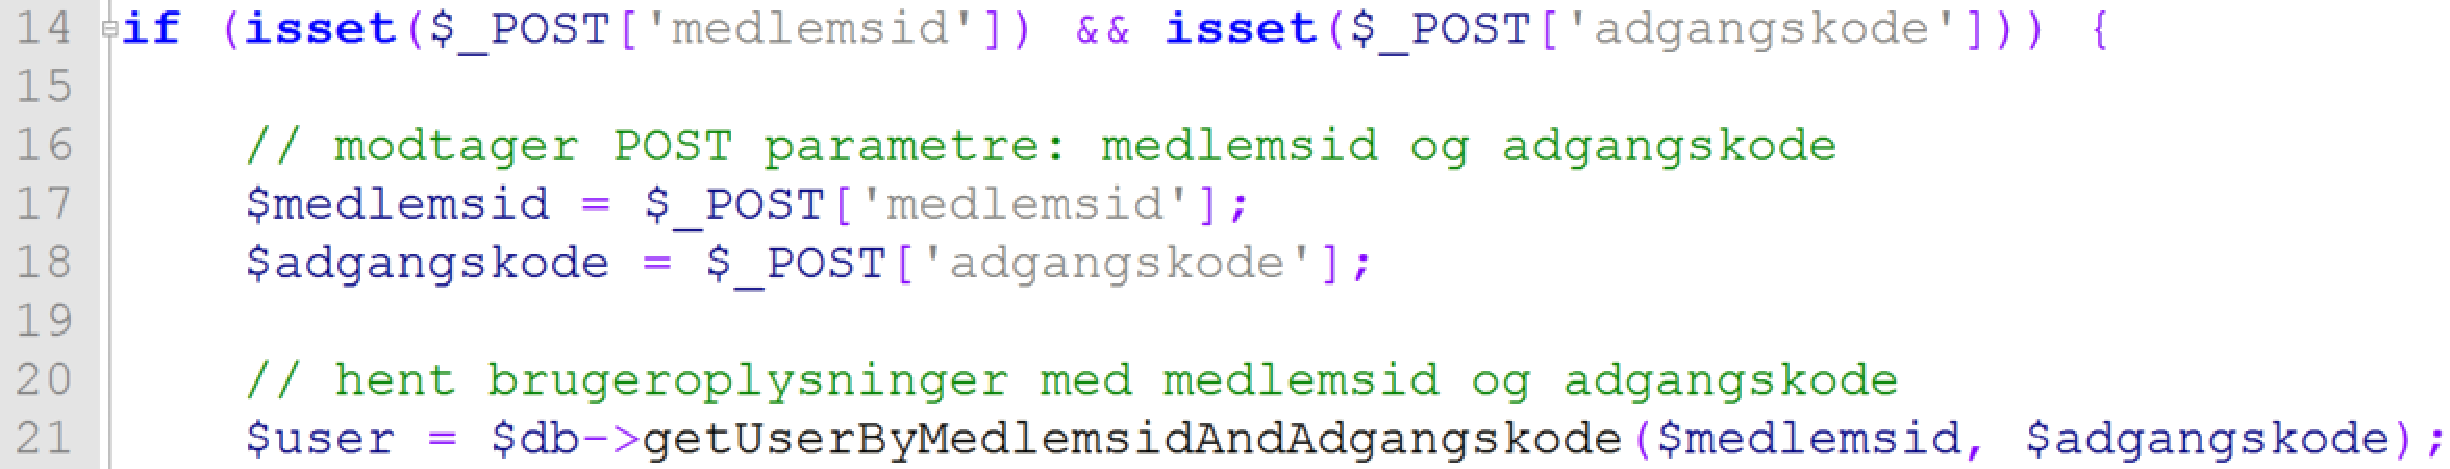
\includegraphics[width=1\textwidth]{figures/imple/phplogind}
\caption{Udklip af log ind php-script, hvor medlemsid samt adgangskode modtages og indsættes i tilhørende variabler, der benyttes i et funktionskald.}
\label{fig:phplogind}
\end{figure}

\noindent
Dette udklip viser, hvordan koden modtages og gemmes i nye variabler. Værdierne gemmes i et associativt array, der ved hjælp af en POST-metode gør det muligt at overføre data til et andet script, \textit{db\_functions.php}, hvori SQL-kommandoer udføres \cite{w3schools2017}. Linje 21 viser, hvordan variablerne benyttes i et funktionskald, der eksekveres i \textit{db\_functitons.php}. Af \autoref{fig:phplogindsql} ses et udklip af denne funktion.

\begin{figure} [H]
\centering
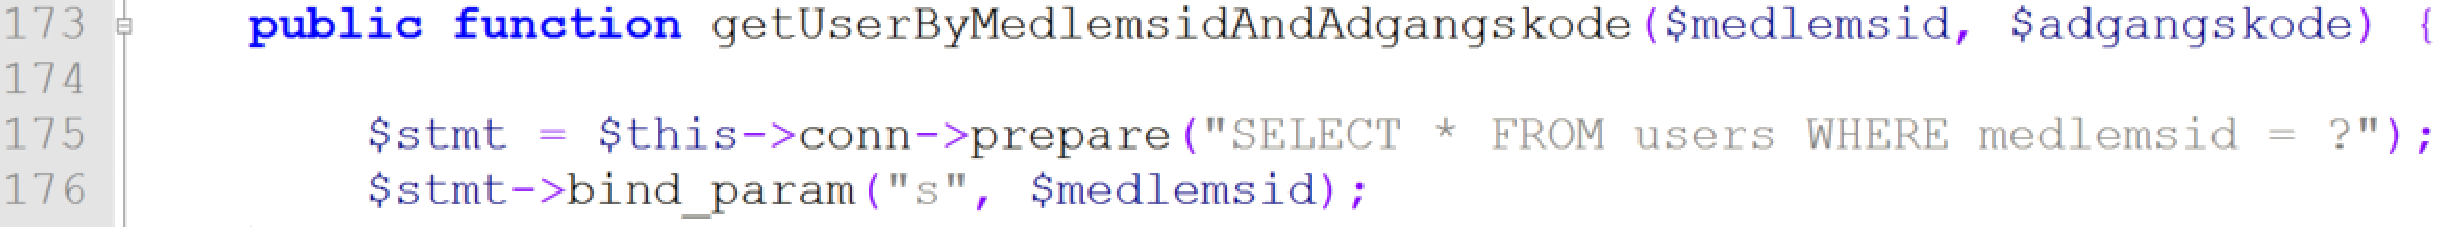
\includegraphics[width=1\textwidth]{figures/imple/phplogindsql}
\caption{Udklip af php-scripts for funktionen log ind. Herunder ses SQL-kommandoen for denne funktion.}
\label{fig:phplogindsql}
\end{figure}

\noindent
Det ses af \autoref{fig:phplogindsql}, hvordan en SQL-kommando udføres. Den viste SQL-kommando henter alt fra tabellen \textit{users} tilhørende medlemsid'et i databasen, der er lig spørgsmåltegn. Spørgsmåltegnet markerer et bindingspunkt, hvorpå en parametre kan tilknyttes. Parameteren, der bindes på ved brug af \textit{bind\_param}, fremgår af linje 176, hvoraf \textit{"s"} indikerer, at medlemsid'et er af typen string. I dette tilfælde valideres log ind-informationerne førend user returneres til log ind php-scriptet, der håndterer user, hvilket fremgår af \autoref{fig:phplogindresp}.


\begin{figure} [H]
\centering
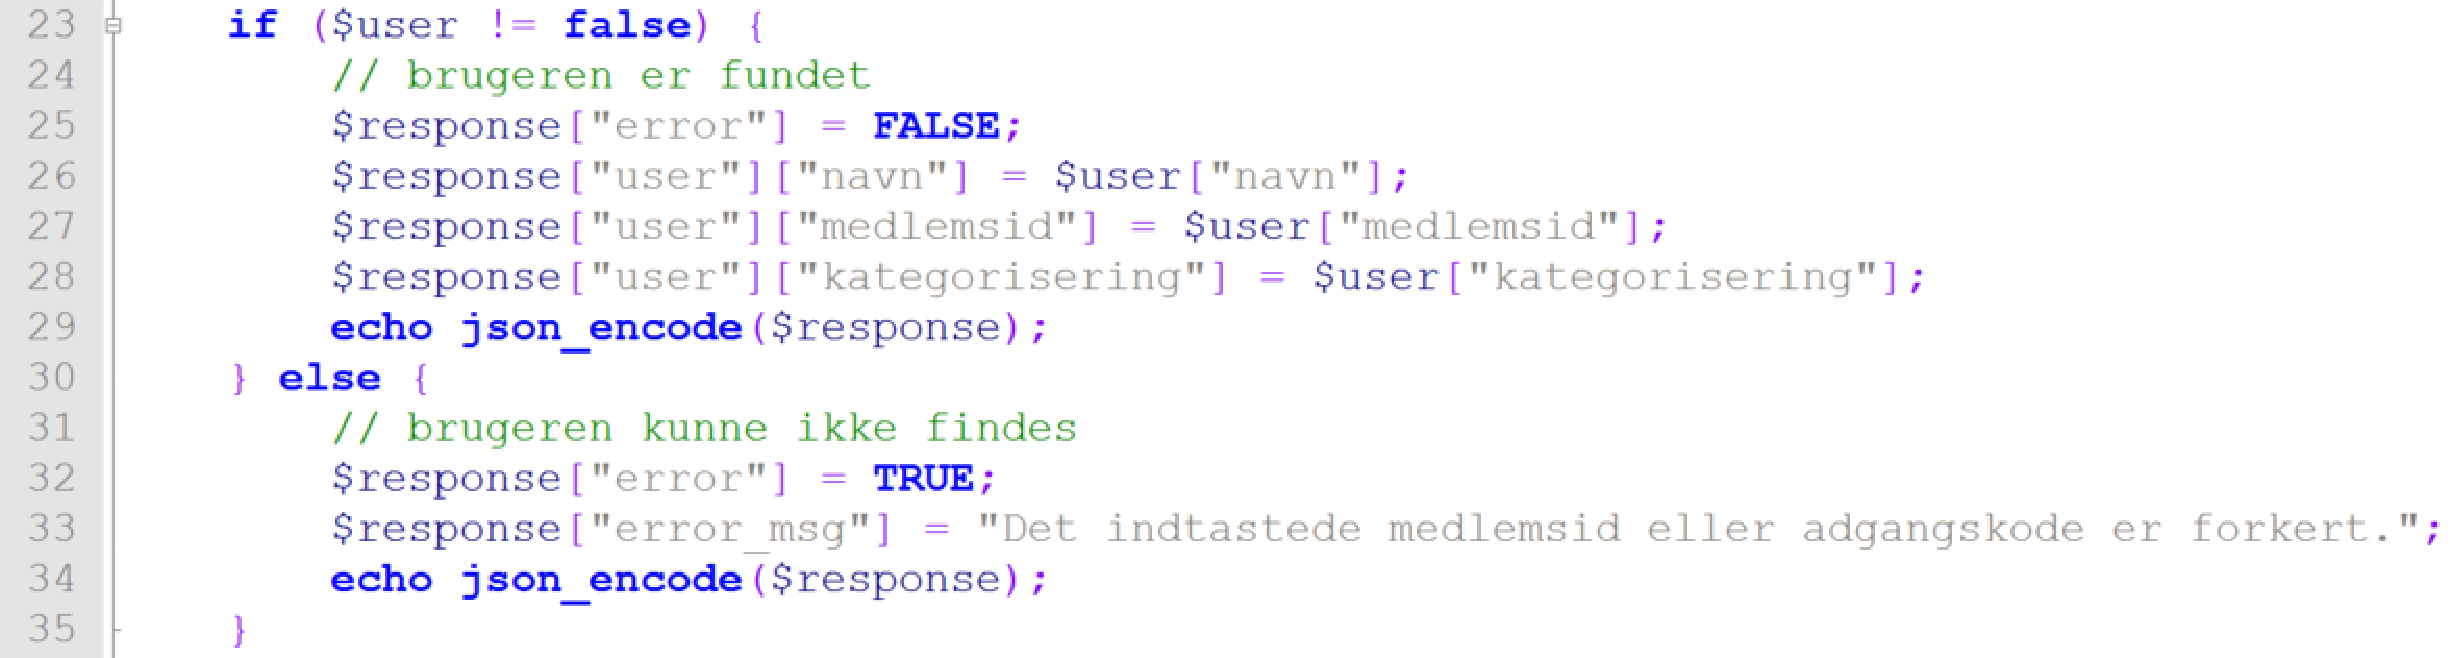
\includegraphics[width=1\textwidth]{figures/imple/phplogindresp}
\caption{Udklip af php-scripts, hvori user håndteres og sendes til app'en.}
\label{fig:phplogindresp}
\end{figure}

\noindent
Som det ses af \autoref{fig:phplogindresp} opstilles if/else statement, der håndterer, hvorvidt \textit{user} returneres. Hvis \textit{user} returneres bliver brugerdata gemt i \textit{response}, der sendes tilbage til app'en som en JSON repræsentation. Returneres \textit{user} ikke, gemmes en fejlmeddelelse i \textit{response}, der ligeledes sendes til app'en som en JSON repræsentation. 

Der er i javakoden opsat en \textit{Response.listener}, der lytter efter respons. Ved respons oprettes et nyt JSON objekt, hvori responset lagres, således dette kan benyttes i app'en. 